\chapter{Parameter Selection}

When choosing the parameters to train the support vector machine, we decided to expand on the data available from the image. By applying certain filters to the image, it is possible to expand on the features of the image without requiring manual editing of the image.

\section{X and Y Coordinates}
Perhaps the most obvious parameters to use are the X and Y-coordinates of each pixel.  The door area is confined to two very specific, continuous areas of the image; the boundaries of this image, however, are not simple, and to satisfactorily represent them, a very high number of sample points would be required.

\section{L*a*b* Colour Values}
Another, simpler observation is that the door largely consists of a single colour: brown.  There are, of course, other brown regions in the image, and there are considerable variations in the shades of brown throughout the door, but this provides a decent guess.  

This observation can be further strengthened by representing the colours of image pixels in terms of luminance and chrominance channels, as specified by the CIELAB (L*a*b*) colour system, which is designed to closely model human visual perception.  It consists of three channels: L*, the luminance channel (where 0 is black, and 100 is diffuse white); a*, the red/magenta-green channel (where positive values are red, and negative are green); and b*, the blue-yellow channel (where positive values are yellow, and negative values are blue) ~\citep{berns2000billmeyer}. The conversion from sRGB pixel values to L*a*b* values is well-known, and is performed in the following manner ~\citep{mclaren1976xiii}.

First, the CIE XYZ tristimulus values are obtained from the sRGB values. sRGB component values R$_{srgb}$, G$_{srgb}$, and B$_{srgb}$ are normalized by dividing by 255 to achieve values in the range 0 to 1. Then, for each C$_{srgb}$, where C $\in$ R, G, B:

\begin{eqnarray}
C_{linear} = \left\{
  \begin{array}{l l}
  	\frac{C_\mathrm{srgb}}{12.92}, & C_\mathrm{srgb}\le0.04045\\
	\left(\frac{C_\mathrm{srgb}+a}{1+a}\right)^{2.4}, & C_\mathrm{srgb}>0.04045
  \end{array} \right. 
\end{eqnarray}
where a = 0.055.
\begin{eqnarray}
\begin{bmatrix}
X\\Y\\Z\end{bmatrix}=
\begin{bmatrix}
0.4124&0.3576&0.1805\\
0.2126&0.7152&0.0722\\
0.0193&0.1192&0.9505
\end{bmatrix}
\begin{bmatrix}
R_\mathrm{linear}\\ 
G_\mathrm{linear}\\ 
B_\mathrm{linear}
\end{bmatrix}
\end{eqnarray}
Next, the tristimulus values are converted to CIELAB values:
%\begin{align*}
\begin{eqnarray}
\left.
  \begin{array}{l l}
   L^\star & = 116 f(Y/Y_n) - 16\\
   a^\star & = 500 \left[f(X/X_n) - f(Y/Y_n)\right]\\
   b^\star & = 200 \left[f(Y/Y_n) - f(Z/Z_n)\right]
  \end{array} \right. 
\end{eqnarray}
%\begin{array}{1 1}
%	L^\star & = 116 f(Y/Y_n) - 16
%	a^\star & = 500 \left[f(X/X_n) - f(Y/Y_n)\right]
%	b^\star & = 200 \left[f(Y/Y_n) - f(Z/Z_n)\right]
%	\end{array}
%	\right. 
%\end{eqnarray}
%\end{align*}
where 
\begin{eqnarray}
f(t) = \left\{
  \begin{array}{l l}
  t^{1/3} & \text{if } t > (\frac{6}{29})^3 \\
  \frac13 \left( \frac{29}{6} \right)^2 t + \frac{4}{29} & \text{otherwise}
\end{array} \right. 
\end{eqnarray}
and Xn, Yn and Zn are the tristimulus values of the reference white point.  In this case, as defined for the sRGB gamut:
\begin{eqnarray}
\begin{array}{l l}
X_{n} = 0.3127\\
Y_{n} = 0.3290\\
Z_{n} = 0.3583
\end{array}
\end{eqnarray}
The L*, a*, and b* channels of the source image after it has been converted from sRGB in this manner may be observed in.

\begin{figure}[h]
        \centering
        \begin{subfigure}[b]{0.33\textwidth}
                \centering
                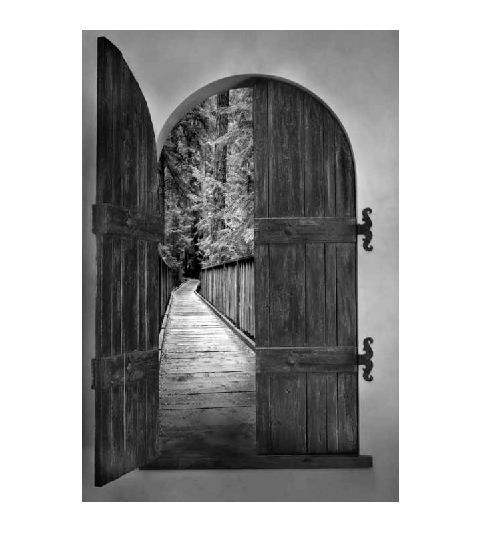
\includegraphics[width=2.6in]{23_LAB_Lchannel}
                \caption{100 Sample points}
                \label{fig:23_LAB_Lchannel}
        \end{subfigure}%
        \begin{subfigure}[b]{0.33\textwidth}
                \centering

                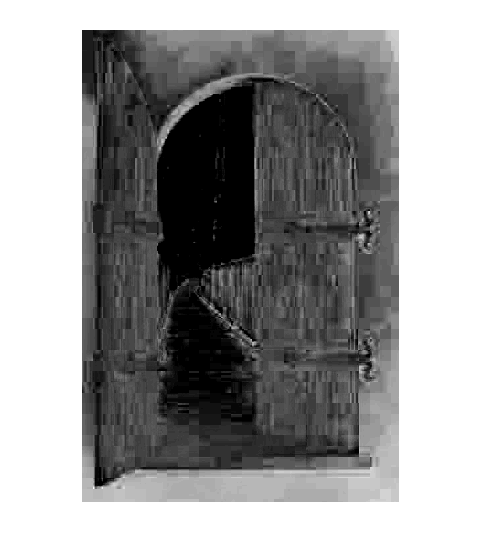
\includegraphics[width=2.6in]{24_LAB_achannel}
                \caption{3000 Sample points}
                \label{fig:24_LAB_achannel}     
        \end{subfigure}
        \begin{subfigure}[b]{0.33\textwidth}
                \centering
                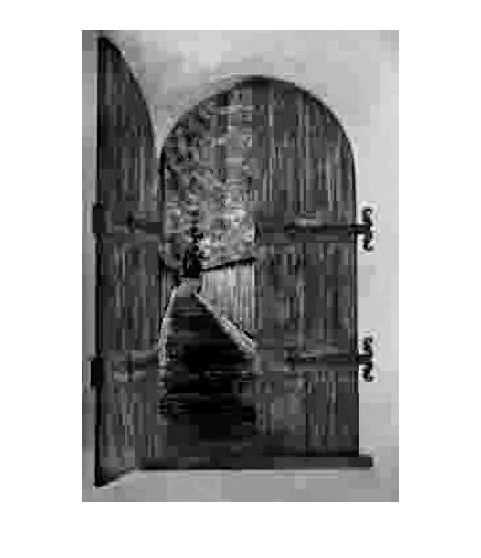
\includegraphics[width=2.6in]{25_LAB_bchannel}
                \caption{6000 Sample points}
                \label{fig:25_LAB_bchannel}     
        \end{subfigure}
        \caption{Results of Differing sample points}\label{fig:labchannels}
\end{figure}

Because the L*a*b* colour space is designed for perceptual uniformity, the perceived colour difference between any two points is fairly accurately defined by the Euclidian distance between them, as specified in the CIELAB $\Delta E_{ab}^*$ 1976 standard:
\begin{equation}
\Delta E_{ab}^* = \sqrt{ (L^*_2-L^*_1)^2+(a^*_2-a^*_1)^2 + (b^*_2-b^*_1)^2 }
\end{equation}
It should be noted that the square of this function is of a very similar form to the RBF kernel function, which also features the Euclidian distance between samples:

\begin{equation}
K(\mathbf{x}, \mathbf{x'}) = \exp\left(-\frac{||\mathbf{x} - \mathbf{x'}||_2^2}{2\sigma^2}\right)
\end{equation}
Therefore, with appropriate training data, the RBF kernel function will loosely approximate the $\Delta E_{ab}^*$ function.

  Preserving the luminance of the image in a channel of its own is also beneficial for another reason. This $L^*$ channel contains the most perceptually important colour information; it may be thought of as a greyscale version of the image, and indeed is a popular choice for simple greyscale conversion. For this image in particular, most regions of the door appear to have similar brightness levels, a feature that would be nearly impossible to infer by using the RGB colour values instead.

\section{Gaussian Blurred L*a*b* Colour Values}
The L*a*b* colour values of each pixel provide a good deal of useful information about the location of the pixel, as the colour value of neighbouring pixels are very likely to be similar.  However, this is not always the case, as parts of the image may contain high-frequency detail.  To compensate for these anomalies, the average colour values of a small surrounding pixel area may be used. Specifically, a Gaussian low-pass filter may be used on the image's L*a*b* pixel values.  

A Gaussian filter of large radius size places a higher weighting on neighbouring pixels at a greater distance from the pixel of interest; a smaller radius better preserves the colour data of the pixel of interest at the expense of not including data from more distant neighbours.  For this application, a Gaussian filter with a circular radius of 5 pixels was arbitrarily chosen as a suitable compromise between the two. 

\section{Sobel Values}
Horizontal and vertical Sobel edge-detection filters were also used to pre-process pixel data. They are defined as follows:

$$ \mathbf{G}_x = 
\begin{bmatrix} 1 & 0 & -1 \\
2 & 0 & -2 \\
1 & 0 & -1 
\end{bmatrix} * \mathbf{A}
\quad
\mbox{and}
\quad   
\mathbf{G}_y = \begin{bmatrix} 
1 & 2 & 1  \\
\ \ 0 & \ \ 0 & \ \ 0 \\
-1 & -2 & -1 
\end{bmatrix} * \mathbf{A}
$$
where $A$ represents the $L^*$ channel of the image.

These filters assign each pixel a value corresponding to the amount of local pixel value change along the $x$ and $y$ directions, respectively.  A high Sobel value indicates that a pixel occurs in an area of the image that has pronounced colour change; under these circumstances, it may be better to place a higher weighting on the colour values of neighbouring pixels than to simply consider the colour values of the pixel itself during classification.  Including Sobel values in the training data set, therefore, allows such a correlation to be inferred, and the classifier should then be able to weight the L*a*b* and Gaussian-blurred L*a*b* values accordingly.